\competentie
{% competentieformulier
	\competentieformulier
	{% toelichting
		Je hebt kennis en vaardigheden die belangrijk zijn voor
		jouw rol als professional in het ict-werkveld. Je kunt de
		kennis die je hebt opgedaan beoordelen op relevantie.
		Op basis daarvan maak je keuzes bij het uitvoeren en
		oplossen van praktijkvraagstukken. Je hanteert daarbij
		een methodische werkwijze, stelt criteria op waaraan
		het resultaat moet voldoen en werkt volgens
		professionele (internationale) ict-standaarden.
		Je hebt een ondernemende houding.
	}
	{% deelcompetenties
		planmatig werken,
		toepassing van (wetenschappelijke) kennis en inzichten,
		kwaliteit leveren,
		ondernemen
	}
	{%
		Proof
	}
	{%
		Deze competentie wordt beoordeeld door een STARR.
	}
	{% verwijzing naar bewijs
		Figure~\ref{fig:terraform},
		Figure~\ref{fig:react},
		Figure~\ref{fig:kubernets}
	}
}
{% bewijzen
	\bewijs
	{% naam
		% TODO 
		Realizeren van de applicatie.
	}
	{% starr
		\starr
		{% betreft
			Kwaliteit leveren,
			ondernemen,
			Planmatig werken
		}
		{% datum
			25-06-2022
		}
		{% situatie
			Een werkgever heeft mij gevraagd een applicatie te Realizeren binnen een tijd.
			De applicatie moet voldoen aan de gestelde eisen van de werkgever.
		}
		{% taak
			De applicatie moet voldoen aan de gestelde eisen van de werkgever.

			De werkgever heeft geen specificaties gegeven over de techologie die gebruikt moet worden voor de applicatie.

		}
		{% activiteiten
			Voor het realizeren van de applicatie heb ik telefonisch contact gehad om duidelijk te bespreken wat de wensen van de werkgever zijn.

			Op basis van deze kriteria kan ik een kwalitatief goede applicatie maken die geschikt is voor de huidige procedure tijdens een spreekuur.

			Omdat de klant niet een specifieke techologie heeft aangegeven heb ik het risico genomen om de applicatie met techologien te maken waar ik zelf nog niet bekwaam mee ben.

			Voor het realizeren van de applicatie ben ik planmatig begonnen met het bestuderen en leren van de inhoud van de cursussen.
			Met deze kennis heb ik daarna de applicatie gerealiseerd.

			Door correct gebruik te maken van kubernetes is het mogelijk het project snel en effiecient te updaten met minimal downtime.

		}
		{% resultaat
			Het resultaat is een applicatie die kan schalen naar gebruik van de user en voldoet aan de vooraf gestelde eisen van de werkgever.

			De applicatie kan snel worden geupdate door gebruik te maken van techologie en hier correct mee om te gaan.
			De applicatie kan grote hoeveelheid verkeer aan dankzij kubernetes.
			Met deze techologie is de applicatie in staat snel op te schalen om zo meer verkeer te kunnen verwerken.

			Door het risico te nemen om nieuwe techologien te gebruiken ben ik nu ook bekwamer bij mijn huidige werkgever dankzij de nieuwe kennis.
		}
		{% reflectie

			Het kiezen voor Kubernetes en terraform heeft het nodig stress geleverd.
			Vooral Kubernetes was erg complex.

			Door planmatig te werken en op tijd te beginnen met het verwerken en leren van de cursussen heb ik genoeg tijd gehad om de applicatie op tijd te kunnen realizeren.

			Het heeft veel tijd gekost om op een correcte manier gebruik te maken van Kubernetes.
			Dit kwam omdat er veel nieuwe methodieken werden geintroduceerd die allemaal met elkaar moeten samen werken.

			Het composeren van alle lossen individuelen delen zoals de load balancer, service en applicatie zelf heeft tijd gekost.

			Ook is het niet gelukt terraform te gebruiken in dit project.
			Ik gebruik dit wel actief bij mijn huidige werkgever met de nieuw behaalde kennis.


			De reden dat het niet gebruikt is in deze applicatie heeft te maken met een verkeerde interpetatie van de techologie.
			Terraform wordt gebruikt voor het managen van cloud componenten en niet voor het managen van een single applicatie.

			Doordat ik in de eerste instantie een verkeerd beeld had van het gebruik van Terraform heb ik hier veel van geleerd.
		}

		{
		}
	}
	{% bewij
		\begin{figure}
			\begin{center}
				
\includegraphics[width=0.95\textwidth]{images/terra.jpg}
			\end{center}
			\caption{Terraform}
			\label{fig:terraform}
		\end{figure}
		\begin{figure}
			\begin{center}
				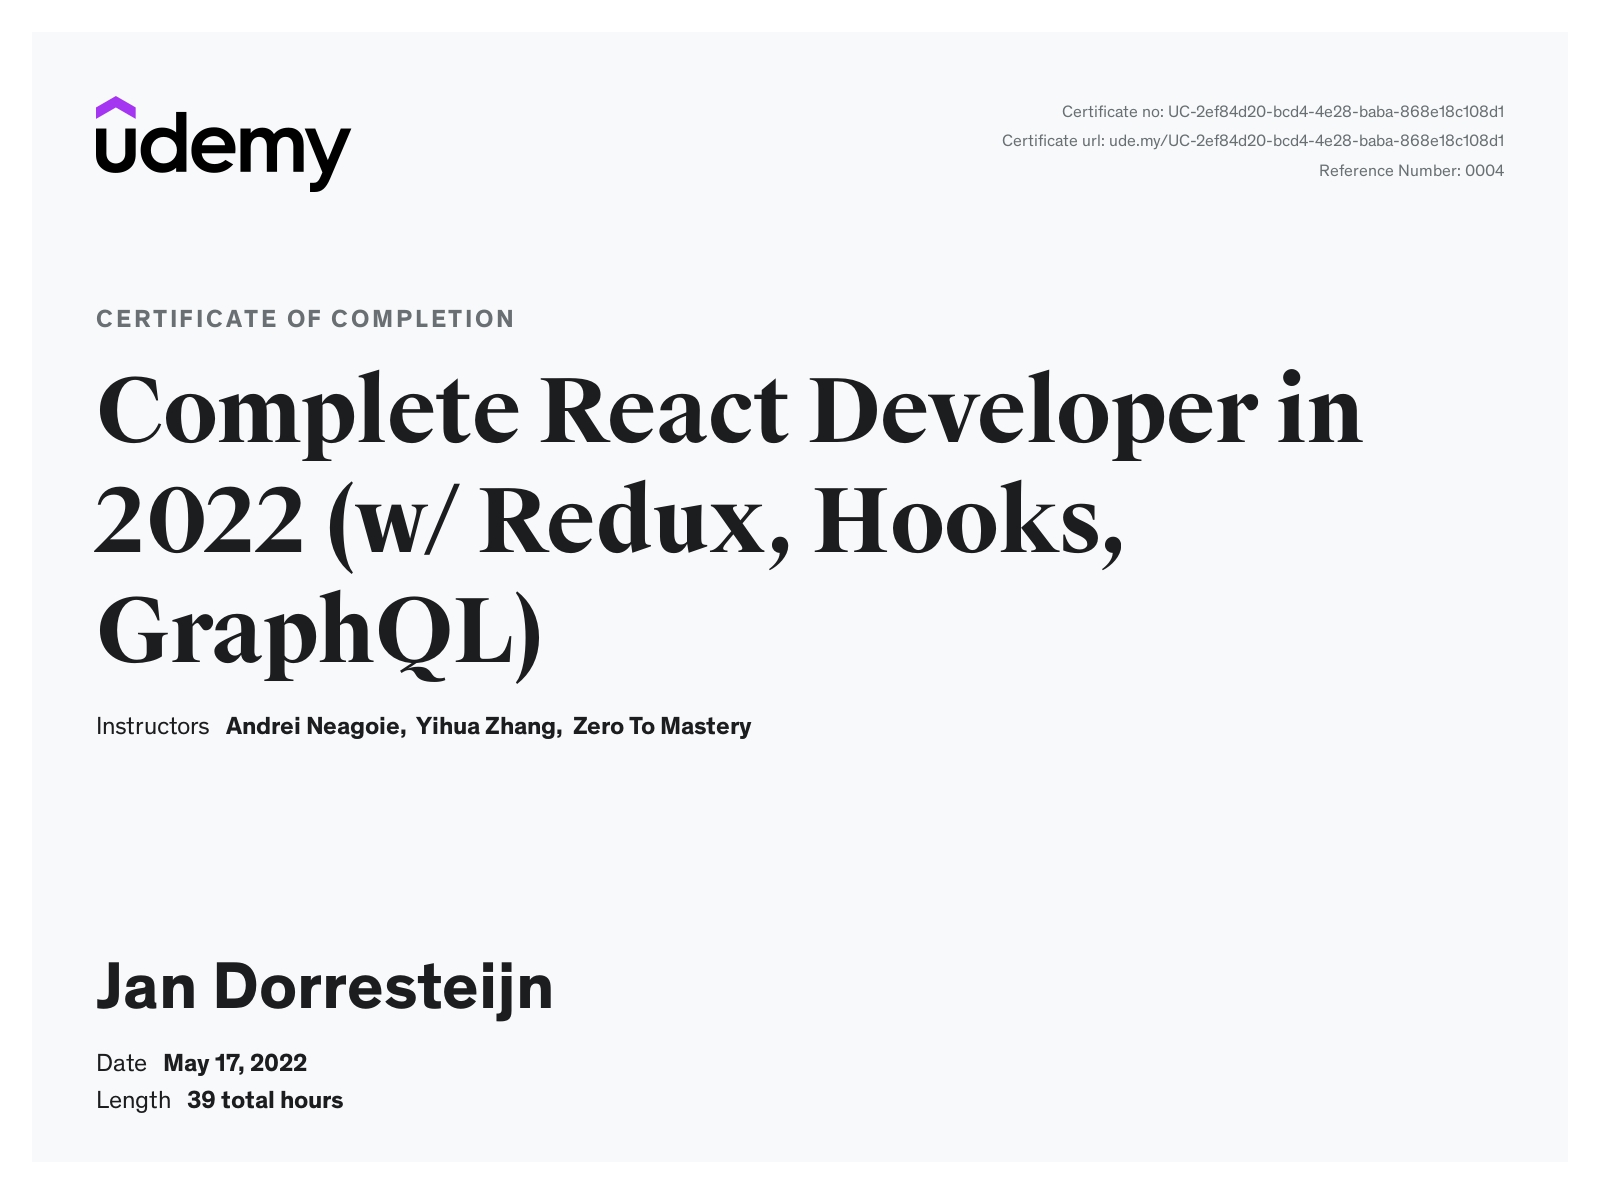
\includegraphics[width=0.95\textwidth]{images/react.jpg}
			\end{center}
			\caption{React}
			\label{fig:react}
		\end{figure}
		\begin{figure}
			\begin{center}
				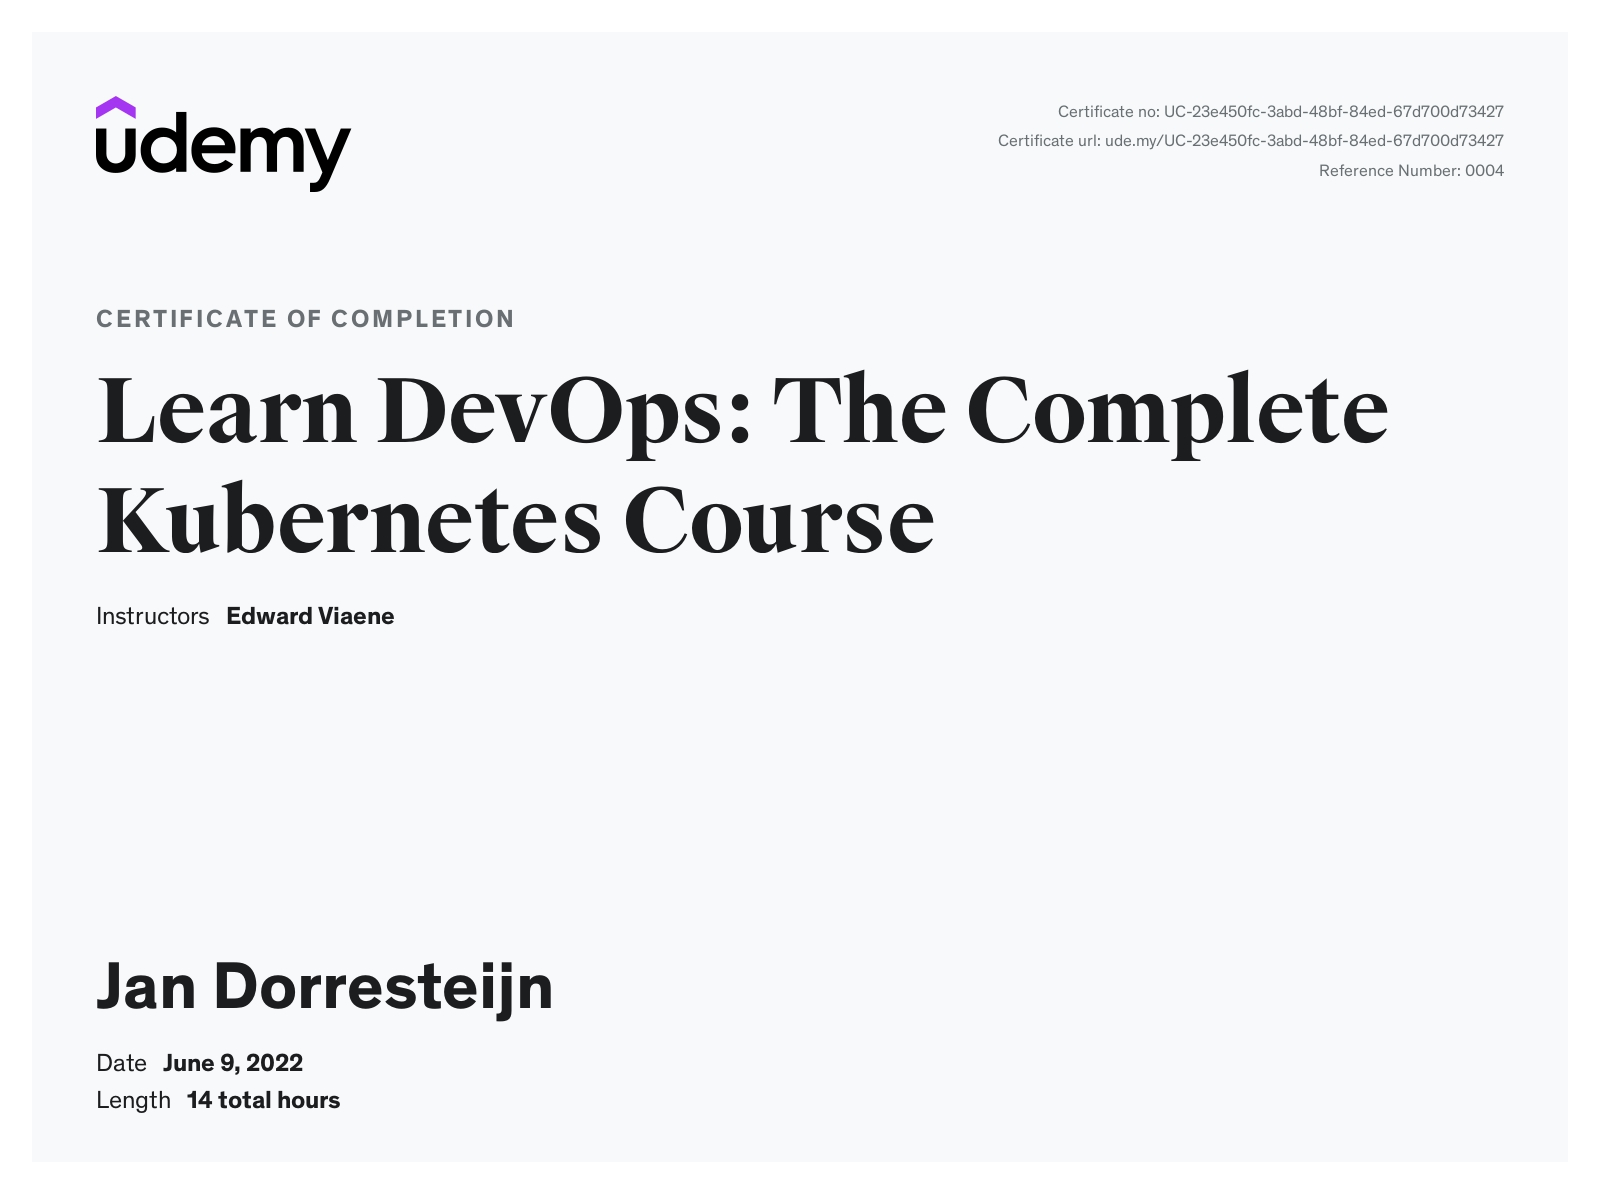
\includegraphics[width=0.95\textwidth]{images/kube.jpg}
			\end{center}
			\caption{Kubernetes}
			\label{fig:kubernets}
		\end{figure}

	},
}

